\documentclass[fr]{../../../eplsummary}

\usepackage{float}
\usepackage{colonequals}
\usepackage[french,ruled,vlined]{algorithm2e}

\graphicspath{{img/}}

\newcommand{\prop}{\langle \textnormal{proposition} \rangle}
\newcommand{\true}{\textnormal{true}}
\newcommand{\false}{\textnormal{false}}
\newcommand{\EP}{\mathcal{E}_P}
\newcommand{\val}[1]{\mathrm{val}_{#1}}
\newcommand{\VAL}[1]{\mathrm{VAL}_{#1}}
\newcommand{\tauto}{{\vDash} \>}
\newcommand{\contra}{{\nvDash} \>}
\providecommand{\lxor}{\oplus}
\newcommand{\logcons}{\Rrightarrow}
\newcommand{\logeq}{\mathrel{\Lleftarrow {} \mspace{-12mu} {} \Rrightarrow}}

\SetKwComment{Comment}{$\triangleright$\ }{}

\hypertitle{Logique et structures discrètes}{5}{INGI}{1101}
{Gilles Peiffer}
{Peter Van Roy}

\part{Logique}
\section{Contexte: la méthode scientifique}
La logique est la science du raisonnement.
Il existe 3 types de raisonnement:
\begin{itemize}
	\item la déduction\footnote{Qu'on étudiera dans ce cours.};
	\item l'induction;
	\item l'abduction.
\end{itemize}
Tout raisonnement fait par un humain
fait partie de l'une de ces trois catégories.
Prenons l'exemple de la méthode scientifique.
L'humain commence en général par émettre une théorie
sur comment fonctionne le monde,
et ce en se basant sur un modèle théorique du monde réel.
Ensuite, à partir de cette théorie,
il est possible de \emph{déduire} les résultats
que devrait avoir une certaine expérience,
si la théorie est juste.
On effectue alors l'expérience,
et on \emph{induit} à partir des résultats
une règle que semble suivre la nature.
Finalement, observant cette règle naturelle,
on la compare avec la théorie proposée,
et si les deux ne sont pas en accord,
on se pose la question ``Pourquoi la nature suit-elle cette règle?''.
La réponse à cette question est une abduction.
\begin{figure}[H]
	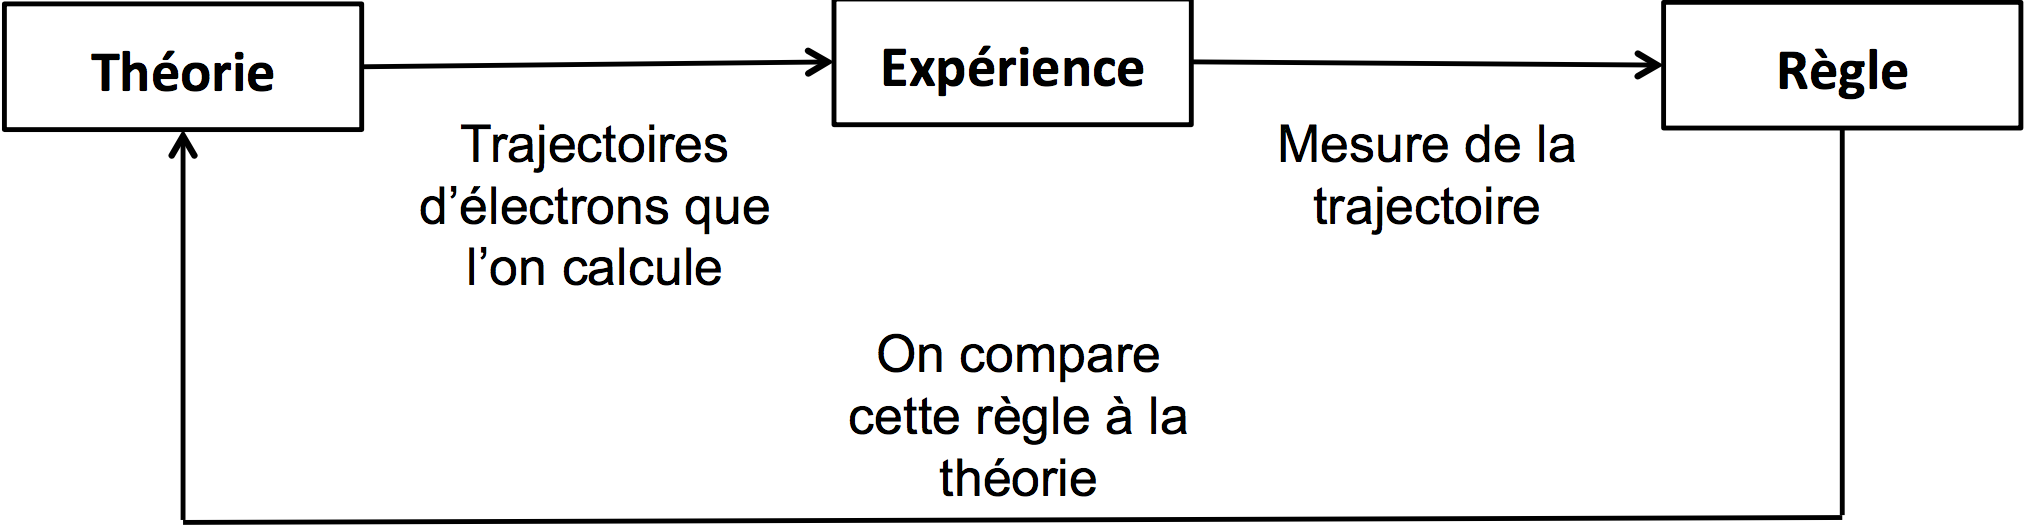
\includegraphics[width=\textwidth]{scientific_method}
	\caption{Un exemple d'utilisation de la méthode scientifique
	pour les lois de Maxwell.
	Notons que ce schéma n'est pas entièrement complet:
	il faudrait séparer la partie ``Expérience'' en deux;
	d'une part tout ce qui est prédiction,
	et d'autre part la mise en place.
	La théorie permet alors de faire les deux.}
	\label{fig:sci_meth}
\end{figure}
\bigbreak
On remarque donc que sur ces trois raisonnements,
uniquement la déduction est un raisonnement sûr,
alors que l'induction et l'abduction ne le sont pas.
\begin{myexem}[Sac de billes]
Un exemple illustrant cette différence
serait un sac rempli de billes colorées.
On suppose que la théorie nous dit
que toutes les billes sont blanches.
On \emph{déduit} donc avec parfaite sûreté
que si on pioche une bille du sac,
elle sera blanche.

Comparons cela avec le cas suivant:
on est en train de piocher des billes du sac,
et on remarque que toutes les billes que l'on pioche sont blanches.
On peut alors \emph{induire} que toutes les billes du sac sont blanches.
Ce raisonnement n'est pas parfaitement sûr,
contrairement à la déduction.

Finalement, supposons que l'on trouve un bille blanche à coté du sac.
On pourrait expliquer cela par le fait que les billes viennent du sac.
Il s'agit d'un raisonnement abductif,
qui n'est d'ailleurs pas sûr.
\end{myexem}

\section{La logique propositionnelle}
La logique propositionnelle
est la plus simple des formes de logique
(on a également la logique des prédicats\footnote{Plus tard dans le cours\dots},
la logique du second ordre, la logique temporelle, la logique modale,\dots).
Elle permet de formaliser les connexions logiques entre des propositions.
\bigbreak
\begin{mydef}[Proposition première]
	Les \emph{propositions premières} sont les ``briques''
	avec lesquelles nous construisons les propositions plus compliquées.
	Elles peuvent soit être vraies (true) ou fausses (false).
	Un exemple pourrait être la phrase
	``La logique est compliquée.\footnote{En l'occurrence,
	cette proposition est fausse\dots}''
	On les dénote avec des lettres majuscules ($A$, $B$,\dots).
\end{mydef}
\begin{mydef}[Proposition logique]
	Une \emph{proposition logique} est alors soit une proposition première,
	soit une combinaison de propositions logiques
	connectées par des connecteurs logiques.
\end{mydef}
L'avantage de cette notation est qu'elle permet de raisonner formellement
sur les propositions logiques.
On peut définir:
\begin{enumerate}
	\item une \emph{syntaxe} (définie par une grammaire)
	qui définit ce qui est une proposition logique et ce qui ne l'est pas;
	\item une \emph{sémantique}
	qui donne un sens à chaque proposition logique;
	\item une \emph{théorie de preuve} permettant,
	en sachant qu'une proposition est vraie,
	de trouver d'autres propositions vraies.
\end{enumerate}
\subsection{Syntaxe}
\label{sec:syntax}
La logique propositionnelle est un \emph{langage formel}.
Ce langage peut être défini à l'aide d'une grammaire sur un \emph{alphabet}.
Cet alphabet est l'ensemble des symboles qui composent une proposition logique:
\begin{itemize}
	\item les lettres majuscules pour les propositions premières: $A$, $B$,\dots;
	\item true et false pour les propositions
	resp. toujours vraie et toujours fausse;
	\item les connecteurs logiques:
	\begin{itemize}
		\item la conjonction (AND): $\land$;
		\item la disjonction (OR): $\lor$;
		\item la négation (NOT): $\lnot$;
		\item l'implication: $\to$ ou $\implies$;
		\item l'équivalence: $\leftrightarrow$ ou $\iff$;
		\item les caractères de ponctuation: $($ et $)$.
	\end{itemize}
	Leur précédence est la suivante:
	\begin{table}[H]
		\[
		\begin{array}{cc}
			\hline
			\textnormal{Connecteur} & \textnormal{Précédence}\\
			\lnot & 1\\
			\land & 2\\
			\lor & 3\\
			\to & 4\\
			\leftrightarrow & 5\\
			\hline
		\end{array}
		\]
	\end{table}
\end{itemize}
La grammaire suivante permet de donner les règles
que doivent respecter les phrases propositionnelles:
\[
\renewcommand{\arraystretch}{1.5}
\begin{array}{rrl}
	\langle \textnormal{identificateur} \rangle & \coloneqq & A \mid B \mid C \mid \dots\\
	\prop &\coloneqq& \true\\
	&\mid& \false\\
	&\mid& \langle \textnormal{identificateur} \rangle\\
	&\mid& \big(\prop\big)\\
	&\mid& \lnot \prop\\
	&\mid& \prop \land \prop\\
	&\mid& \prop \lor \prop\\
	&\mid& \prop \to \prop\\
	&\mid& \prop \leftrightarrow \prop
\end{array}
\]
On remarque qu'uniquement les séquences de symboles
qui respectent cette grammaire
sont des phrases propositionnelles.
\paragraph{Métalangage}
Le métalangage est un deuxième langage utilisé pour parler d'un premier,
dans notre cas, la logique propositionnelle.
Notre métalangage est le français,
auquel on ajoute les notations mathématiques.
Ce concept est important pour distinguer raisonnement formel et informel.
\subsection{Tables de vérité}
La syntaxe développée à la \sectionref{syntax}
permet d'écrire les propositions en logique formelle,
mais ne leur donne pas de sens (vrai ou faux).
Afin de donner un sens aux propositions,
il faut commencer par déterminer
si les propositions premières sont vraies ou fausses.
Pour cela, il y a deux approches:
les \emph{tables de vérité}
et les \emph{interprétations}.
Les propositions logiques sont construites
à partir de propositions plus simples.
Une table de vérité est une façon de partir
des valeurs de différentes propositions
pour déterminer la valeur d'une autre proposition.
Voici les tables de vérité des différents connecteurs logiques
(le connecteur XOR ($p \lxor q$)
est une façon plus simple
d'écrire $\lnot(p \land q) \land (p \lor q)$):
\begin{table}[H]
	\[
	\begin{array}{cc|c|c|c|c|c|c}
		p & q & p \land q & p \lor q & \lnot p & p \to q & p \leftrightarrow q & p \lxor q\\
		\hline
		\true & \true & \true & \true & \multirow{2}{*}{\false} & \true & \true & \false\\
		\true & \false & \false & \true & & \false & \false & \true \\
		\false & \true & \false & \true & \multirow{2}{*}{\true} & \true & \false & \true\\
		\false & \false & \false & \false & & \true & \true & \false
	\end{array}
	\]
\end{table}
\subsection{Interprétations}
On peut également définir si une proposition est vraie ou fausse
en utilisant une \emph{interprétation}.
Soit $\EP$ l'ensemble des propositions premières.
Alors, une interprétation $I$ définit
une fonction de valuation $\val{I} \colon \EP \to \{\true,\false\}$,
qui permet de savoir si ces propositions premières sont vraies ou fausses\footnote{La notation $f \colon A \to B$ signifie ici
que $f$ est une fonction depuis l'ensemble $A$ vers l'ensemble $B$.}.
On pourrait par exemple écrire
\begin{align*}
	\left\{
	\begin{array}{rcl}
		\val{I_1}(P) & = & \true\,,\\
		\val{I_1}(Q) & = & \false
	\end{array}
	\right.
	\quad \textnormal{et} \quad
	\left\{
	\begin{array}{rcl}
		\val{I_2}(P) & = & \true\,,\\
		\val{I_2}(Q) & = & \true\,.
	\end{array}
	\right.
\end{align*}
Il y a donc différentes interprétations possibles,
et chacune d'elles risque de donner un résultat différent.
\bigbreak
À partir de ces fonctions de valuation premières,
on peut définir d'autres fonctions de valuation:
$\VAL{I}$ se définit par rapport à $\val{I}$.
On a ainsi
\begin{align*}
	\VAL{I}(P) &= \val{I}(P)\,,\quad \forall P \in \EP\,,\\
	\VAL{I}(\lnot P) &=
	\left\{
	\begin{array}{l}
		\false \textnormal{ si } \VAL{I}(P) = \true\,,\\
		\true \textnormal{ sinon}\,,
	\end{array}
	\right.\\
	\VAL{I}(P \land Q) &=
	\left\{
	\begin{array}{l}
		\true \textnormal{ si } \VAL{I}(P) = \true \textnormal{ et } \VAL{I}(Q) = \true\,,\\
		\false \textnormal{ sinon}\,,
	\end{array}
	\right.\\
	\VAL{I}(P \lor Q) &=
	\left\{
	\begin{array}{l}
		\true \textnormal{ si } \VAL{I}(P) = \true \textnormal{ ou } \VAL{I}(Q) = \true\,,\\
		\false \textnormal{ sinon}\,.
	\end{array}
	\right.
\end{align*}
\subsection{Les modèles logiques}
Une interprétation est un modèle $M$ pour une certaine théorie si
les propositions premières sont telles
que tous les axiomes de la théorie soient vrais.
\begin{myexem}
	Prenons le cas suivant:
	\begin{align*}
		&L\textnormal{: ``Le cours de logique est facile.'',}\\
		&E\textnormal{: ``L'étudiant a bien étudié.'',}\\
		&R\textnormal{: ``L'étudiant a réussi l'examen de logique.'',}
	\end{align*}
	\[
	\big(L \land E\big) \to R\,.\tag*{Axiome~(1)}
	\]
	Un modèle possible des études supérieures serait donc
	\[
	(L,E,R) = (\true,\true,\true)\,.
	\]
\end{myexem}
On peut donc dire que la théorie est un ensemble de formules
et que le modèle est une interprétation qui satisfait ces formules.
\bigbreak
Soit une formule $p$ aléatoire.
\begin{mydef}[Tautologie]
	Si $p$ est vraie dans toutes les interprétations possibles,
	alors on dit que $p$ est une tautologie ($\tauto p$).
	On a par exemple $p \equiv \big(P \lor \lnot P\big)$.
\end{mydef}
\begin{mydef}[Contradiction]
	Si $p$ est fausse dans toutes les interprétations possibles,
	alors on dit que $p$ est une contradiction ($\contra p$).
	On a par exemple $p \equiv \big(P \land \lnot P\big)$.
\end{mydef}
\begin{mydef}[Contingence]
	Si $p$ n'est ni une tautologie,
	ni une contradiction,
	on dit que $p$ est contingente.
	Par exemple, $p \equiv \big(P \land \lnot Q\big)$.
\end{mydef}
\subsubsection{Conséquence logique}
On note ``$q$ est conséquence logique de $p$''
par $p \logcons q$\footnote{Le Prof. Van Roy
utilise les notations $p \logcons q$ et $p \logeq q$
pour la conséquence et l'équivalence logique.
Cependant, dans la littérature,
on utilise $p \implies q$ et $p \iff q$ pour celles-ci.
Comme le Prof. Van Roy utilise déjà celles-ci
pour la conséquence et l'équivalence matérielles
(qui dans la littérature sont souvent représentées
par $p \to q$ et $p \leftrightarrow q$),
on reprendra donc sa notation,
bien qu'elle soit non standard.}.
Soit $p \vDash q$.
Cela veut dire que si $M$ est modèle de $p$, alors $M$ est aussi modèle de $q$.
On a donc $\tauto (p \to q)$,
car $p \to q$ est toujours vrai.
On peut donc bien écrire $p \logcons q$.
\begin{myexem}
	Soit $p \equiv \big(P \land Q\big)$ et $q \equiv \big(P\big)$.
	On a alors que $p \vDash q$.
\end{myexem}
La conséquence logique $p \logcons q$ fait partie du métalangage,
et n'est donc pas une proposition logique.
\subsubsection{Équivalence logique}
Par un raisonnement similaire,
si on a $p \vDash q$ et $q \vDash p$,
on a également $\tauto (p \to q)$ et $\tauto (q \to p)$.
On peut donc écrire $p \logeq q$.
L'équivalence logique n'est pas non plus une proposition logique
mais fait partie du métalangage.

\section{Preuves en logique propositionnelle}
\begin{mydef}[Preuve]
	Une \emph{preuve} est un raisonnement déductif
	qui démontre si une proposition est vraie ou fausse.
	On distingue les preuves \emph{formelles} et \emph{informelles}.
	\begin{itemize}
		\item Une \emph{preuve formelle}
		est un raisonnement en langage naturel,
		parfois augmenté avec des notations mathématiques.
		\item Une \emph{preuve informelle}
		est un raisonnement mathématique
		qui formalise le raisonnement déductif.
	\end{itemize}
\end{mydef}
\begin{myrem}
	``On peut prouver $q$ à partir de $p$'' se note $p \vdash q$.
\end{myrem}
\subsection{Preuve avec table de vérité}
La preuve formelle la plus simple est une table de vérité.
On fait un tableau avec $2^n$ lignes,
où $n$ est le nombre de propositions premières,
et pour chaque ligne,
on prouve une équivalence.
Cette méthode de preuve a l'inconvénient d'être très longue,
et en pratique elle n'est pas réellement utile
au-delà d'une centaine de propositions premières.
On appelle ces programmes (qui ont des heuristiques supplémentaires)
des \textsc{SAT} solvers.
Elle n'est également pas valable pour la logique des prédicats.
\subsection{Preuve transformationnelle}
Une preuve transformationnelle est une séquence de transformations
\[
p_1 \logeq p_2 \logeq \cdots \logeq p_n
\]
dans laquelle on a toujours $p_i \logeq p_{i+1}$.
Une preuve transformationnelle est aussi un objet mathématique en métalangage.
On utilise pour ceci des ``lois'' de transformation,
c'est-à-dire des équivalences connues.
\begin{table}[H]
\renewcommand\arraystretch{1.5}
\centering
\begin{tabular}{rcl@{\qquad}l}
	\hline
	$p$ & $\logeq$ & $p \lor p$ & Idempotence de $\lor$ \\
	$p$ & $\logeq$ & $p \land p$ & Idempotence de $\land$ \\
	$p \lor q$ & $\logeq$ & $q \lor p$ & Commutativité de $\lor$ \\
	$p \land q$ & $\logeq$ & $q \land p$ & Commutativité de $\land$ \\
	$(p \lor q) \lor v$ & $\logeq$ & $p \lor (q \lor v)$ & Associativité de $\lor$ \\
	$(p \land q) \land v$ & $\logeq$ & $p \land (q \land v)$ & Associativité de $\land$ \\
	$\lnot \lnot p$ & $\logeq$ & $p$ & Double négation \\
	$p \to q$ & $\logeq$ & $\lnot p \lor q$ & Implication \\
	$\lnot(p \land q)$ & $\logeq$ & $\lnot p \lor \lnot q$ & 1\ieme{} loi de De Morgan \\
	$\lnot(p \lor q)$ & $\logeq$ & $\lnot p \land \lnot q$ & 2\ieme{} loi de De Morgan \\
	$p \leftrightarrow q$ & $\logeq$ & $(p \to q) \land (q \to p)$ & Équivalence \\
	$(p \land q) \lor r$ & $\logeq$ & $(p \lor r) \land (q \lor r)$ & Distributivité de $\lor$ \\
	$(p \lor q) \land r$ & $\logeq$ & $(p \land r) \lor (q \land r)$ & Distributivité de $\land$ \\
	\hline
\end{tabular}
\caption{Lois de transformation.}
\label{tab:trans}
\end{table}
Pour réellement utiliser ces lois,
on rajoute deux lois supplémentaires:
\begin{itemize}
	\item La \emph{transitivité de l'équivalence}.

	Si $p \logeq q$ et $q \logeq r$,
	alors $p \logeq r$.
	\item Le \emph{principe de substitution}.

	On peut remplacer une sous-formule
	par une autre sous-formule équivalente
	à l'intérieur d'une formule.
\end{itemize}

\subsection{Preuve déductive}
Une preuve déductive est un objet mathématique
qui formalise une séquence de pas de raisonnement simples.
Chaque pas doit être justifié
avec le nom de la règle ou la loi qui est utilisée.
Les pas utilisent trois techniques de raisonnement différentes:
les équivalences logiques,
les règles d’inférence et
les schémas de preuve.
\subsubsection{Équivalences logiques}
Les équivalences logiques sont les mêmes
que celles données dans la \tabref{trans}.
\subsubsection{Règles d'inférence}
Contrairement aux preuves transformationnelles, les règles d'inférence
ont une direction:
elles commencent par les prémisses et terminent par une conclusion.
On utilise un raisonnement informel pour justifier les règles.

\begin{table}[H]
\centering
\renewcommand{\arraystretch}{1.5}
\begin{tabular}{cl@{\qquad\qquad}cl}
	\hline
	$\begin{array}{c}
	p \\
	q \\
	\hline
	p \land q
	\end{array}$ & Conjonction & $\begin{array}{c}
	p \\
	\lnot p \\
	\hline
	q
	\end{array}$ & Contradiction \\
	&&&\\
	$\begin{array}{c}
	p \land q \\
	\hline
	p
	\end{array}$ & Simplification & $\begin{array}{c}
	p \\
	\hline
	p \lor q
	\end{array}$ & Addition \\
	&&&\\
	$\begin{array}{c}
	p \leftrightarrow q\\
	q \leftrightarrow r\\
	\hline
	p \leftrightarrow r
	\end{array}$ & Transitivité de l'équivalence & $\begin{array}{c}
	p \lor q\\
	\lnot p \\
	\hline
	q
	\end{array}$ & Syllogisme disjoint \\
	&&&\\
	$\begin{array}{c}
	p \to q \\
	p \\
	\hline
	q
	\end{array}$ & Modus ponens & $\begin{array}{c}
	p \to q \\
	\lnot q \\
	\hline
	\lnot p
	\end{array}$ & Modus tollens \\
	&&&\\
	$\begin{array}{c}
	p \leftrightarrow q \\
	\hline
	q \leftrightarrow p
	\end{array}$ & Loi d'équivalence & $\begin{array}{c}
	\lnot \lnot p \\
	\hline
	p
	\end{array}$ & Double négation \\
	\hline
\end{tabular}
\caption{Ensemble des règles d'inférence utilisées.}
\label{tab:inference}
\end{table}

\subsubsection{Schémas de preuve}
En plus des équivalences logiques et des règles d'inférence,
on a deux schémas de preuve
qui formalisent des techniques de raisonnement plus abstraites:
le théorème de déduction et la démonstration par l'absurde.
En général, on met ces preuves dans des schémas comme celui en \figuref{proof}.
\begin{figure}[H]
\centering
\begin{tabular}{ccc}
	& Formule & Justification \\
	\hline
	1. & $s$ & $\cdots$ \\
	2. & $\cdots$ & $\cdots$ \\
	\multirow{3}{*}{$\vdots$} & \multirow{3}{*}{$\vdots$} & \multirow{3}{*}{$\vdots$} \\
	&&\\
	&&\\
	$n$. & $t$ & $\cdots$\\
	\hline
\end{tabular}
\caption{Le squelette d'une preuve en logique propositionnelle.}
\label{fig:proof}
\end{figure}
\paragraph{Théorème de déduction (preuve conditionnelle)}
Supposons $s$ vraie.
C'est notre hypothèse.
Elle s'ajoute donc aux prémisses utilisées dans la preuve.
Ensuite, on fait une preuve de $t$.
On peut construire une preuve (objet mathématique) de $t$ en commençant de $s$.
On note ceci $s \vdash t$.
\[
\begin{array}{lcr}
	p,\dots,r,s & \vdash & t \\
	\hline
	p,\dots,r & \vdash & s \to t
\end{array}
\]
On a évacué l'hypothèse.
\paragraph{Démonstration par l'absurde (preuve par contradiction)}
Également appelée \emph{reductio ad absurdum}.
On suppose nos prémisses $p,\dots,q$ sans contradiction.
On rajoute $r$ aux prémisses.
Si on peut prouver $s$ et $\lnot s$,
cela signifie que $r$ rend les prémisses inconsistantes.
\[
\begin{array}{lcr}
	p,\dots,q,r & \vdash & s \\
	p,\dots,q,r & \vdash & \lnot s\\
	\hline
	p,\dots,q & \vdash & \lnot r
\end{array}
\]
\subsection{Algorithme de preuve}
Les preuves manuelles de la section précédente
ont un grand défaut:
elles sont extrêmement lentes.
Afin de diminuer le temps nécessaire pour prouver une équivalence logique,
on peut définir un algorithme de preuve,
qui est une automatisation d'une démonstration par l'absurde
qui est basée sur une seule règle,
la \emph{résolution}.

\subsubsection{Tranformation en forme normale conjonctive}

Toute formule logique peut être transformée en une formule équivalente,
qui est une conjonction de disjonctions.
C'est la forme normale conjonctive (\textsc{FNC}).
On peut également définir une forme similaire,
la \textsc{FND} (forme normale disjonctive),
qui est donc une disjonction de conjonctions.

\paragraph{Terminologie}
Afin de faciliter la discussion autour des formes normales,
on introduit la terminologie suivante:
\begin{itemize}
	\item Un \emph{littéral} $L$ est soit une proposition première,
	soit la négation d'une proposition première.
	\item Une \emph{clause} $C$, en \textsc{FNC},
	est une disjonction de littéraux.
	On écrit
	\begin{align*}
	C &\equiv \bigvee\limits_{i = 1}^{n} L_i\\
	&\equiv L_1 \lor L_2 \lor \dots \lor L_n\,.
	\end{align*}
	En \textsc{FNC}, on a souvent des conjonctions de clauses,
	c'est-à-dire des formules de la forme
	\begin{align*}
	\bigwedge\limits_{i=1}^{m} C_i &\equiv \bigwedge\limits_{i = 1}^{m} \bigvee\limits_{j = 1}^{n_i} L_{ij}\\
	&\equiv \big(L_{11} \lor \dots \lor L_{1n_1}\big) \land \dots \land \big(L_{m1} \lor \dots \lor L_{mn_m}\big) \,.
	\end{align*}
\end{itemize}

\paragraph{Algorithme de normalisation}
Pour mettre sous \textsc{FNC} une formule logique quelconque,
on utilise l'algorithme suivant:
\begin{enumerate}
	\item éliminer les implications et équivalences matérielles
	($\to$ et $\leftrightarrow$)
	en les remplaçant par des formules équivalentes;
	\item déplacer les négations vers l'intérieur
	(jusqu'aux propositions premières)
	en utilisant les formules de De Morgan;
	\item déplacer les disjonctions ($\lor$) vers l'intérieur
	en utilisant les lois distributives;
	\item simplifier en éliminant les formes $(P \lor \lnot P)$
	dans chaque disjonction.
\end{enumerate}

\subsubsection{Résolution}
La règle de résolution est l'unique règle d'inférence utilisée
dans les algorithmes de preuve.
Elle s'écrit comme suit:
\[
\begin{array}{l@{}c@{}r}
	p_1 & {} \lor {} & q\\
	p_2 & {} \lor {} & \lnot q\\
	\hline
	p_1 & {} \lor {} & p_2
\end{array}
\]
\begin{myrem}[La résolution préserve les modèles]\leavevmode
\begin{proof}
	Soient
	\begin{align*}
		p &\equiv \bigwedge\limits_{i=1}^{2} C_i\,,\\
		C_1 &\equiv p_1 \lor q\,,\\
		C_2 &\equiv p_2 \lor \lnot q\,,\\
		r &\equiv p_1 \lor p_2\\
		&\equiv \left(C_1 - \{P\}\right) \lor \left(C_2 - \{\lnot P\}\right)\,.
	\end{align*}
	$r$ est une nouvelle disjonction à partir de deux autres disjonctions.
	Prouvons que $r$ est toujours vrai ($\{C_1, C_2\} \vDash r$).
	On utilise pour cela la sémantique,
	une preuve en métalangage qui n'est donc pas formalisée.

	Si
	\[
	\left\{
	\begin{array}{c}
		\VAL{I}(C_1) = \true\,,\\
		\VAL{I}(C_2) = \true\,,
	\end{array}
	\right.
	\]
	alors $I$ est modèle de $\{C_1, C_2\}$.

	On voit que c'est le cas,
	car on a toujours soit $\VAL{I}(q) = \true$
	et donc $\VAL{I}(p_2) = \true$,
	ou bien $\VAL{I}(q) = \false$
	et donc $\VAL{I}(p_1) = \true$.
	$r$ est donc toujours vrai.
\end{proof}
\end{myrem}

\subsubsection{Pseudocode}

Prenons des axiomes $C_i$ en \textsc{FNC}:
\begin{align*}
C_i &= \bigvee\limits_{i=1}^{n} L_i\,,\\
L_i &= P \textnormal{ ou } \lnot P\,,
\end{align*}
et un théorème à prouver, $C$.
On veut donc démontrer
\[
\{C_1, \dots,C_n\} \vdash C\,.
\]
On sait que
\[
\{C_1, \dots, C_n\} \vDash C \iff \{C_1, \dots, C_n, \lnot C\} \vDash \false\,.
\]
Il suffit donc de démontrer que $\mathcal{S} = \{C_1, \dots, C_n, \lnot C\}$
est inconsistant.
Pour faire cela,
l'algorithme de preuve combine les éléments de $\mathcal{S}$
grâce à la résolution,
jusqu'à ce qu'on arrive à une contradiction,
ou qu'il n'y ait plus de possibilité d'utiliser la résolution.
Dans le premier cas,
nous avons prouvé $C$.
Dans le second,
$C$ est improuvable.

\begin{algorithm}[H]
\DontPrintSemicolon
\KwData{$C_1,\dots,C_n$ les clauses, et $C$ le théorème à prouver.}
\KwResult{Si oui ou non $C_1, \dots, C_n \vdash C$.}
\Begin{
	$\mathcal{S} \gets \{C_1, \dots, C_n, \lnot C\}$\;
	\While{$\false \notin \mathcal{S}$ et
	$\exists C_i, C_j \in \mathcal{S}$ telles que $C_i, C_j$
	résolvables et non résolues}{
		choisir $C_1, C_2 \in \mathcal{S}$
		telles que $\exists P \in C_1, \lnot P \in C_2$\;
		calculer $r \gets C_1 - \{P\} \lor C_2 - \{ \lnot P\}$\;
		calculer $\mathcal{S} \gets \mathcal{S} \cup \{r\}$\;
	}
	\eIf{$\false \in \mathcal{S}$}{
		\Return \true \Comment*[r]{$C$ prouvé}
	}{
		\Return \false \Comment*[r]{$C$ improuvable}
	}
}
\caption{Algorithme de preuve\label{algo:proof}}
\end{algorithm}

En plus de prouver l'existence éventuelle d'une preuve,
l'algorithme de preuve nous donne également cette preuve.

\begin{myprop}[Propriétés de l'algorithme de preuve]
	Pour toute théorie $B = \{C_1, \dots, C_n\}$ et théorème $C$,
	l'algorithme de preuve est
	\begin{itemize}
		\item \textbf{Décidable (\emph{decidable}).}
		L'algorithme se termine
		après un nombre fini d'étapes $\forall B,C$.
		\item \textbf{Adéquat (\emph{sound}).}
		Si $B \vdash C$,
		alors $B \vDash C$.
		\item \textbf{Complet (\emph{complete}).}
		Si $B \vDash C$,
		alors $B \vdash C$.
	\end{itemize}

	Le temps d'exécution
	est exponentiel en le nombre de propositions premières
	et de clauses\footnote{Bien que ce temps d'exécution
	puisse être fortement amélioré
	par l'utilisation de diverses heuristiques,
	comme celles utilisées dans les \textsc{SAT} solvers.}.
\end{myprop}
\end{document}
